\documentclass[tikz,border=6pt]{standalone}
\usepackage{amsmath}
\usepackage{xcolor}

\definecolor{blockblue}{HTML}{4A90D9}

\begin{document}
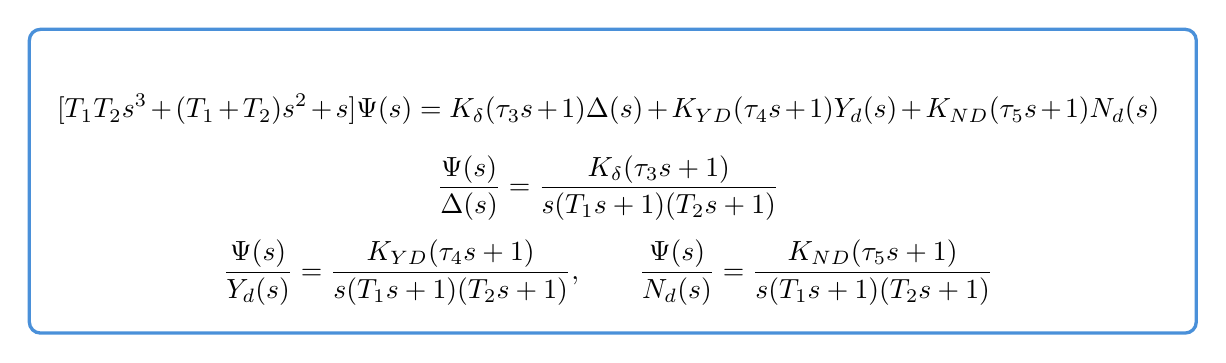
\begin{tikzpicture}[line width=1.2pt]
  \node[
    draw=blockblue,
    rounded corners=4pt,
    inner sep=10pt,
    align=left
  ] at (0,0) {
    \begin{minipage}{14cm}
    \[
    [T_1T_2 s^3 + (T_1+T_2)s^2 + s]\Psi(s)
    =
    K_\delta(\tau_3 s + 1)\Delta(s)
    + K_{YD}(\tau_4 s + 1)Y_d(s)
    + K_{ND}(\tau_5 s + 1)N_d(s)
    \]
    \[
    \frac{\Psi(s)}{\Delta(s)}=
    \frac{K_\delta(\tau_3 s + 1)}{s(T_1s+1)(T_2s+1)}
    \]
    \[
    \frac{\Psi(s)}{Y_d(s)}=
    \frac{K_{YD}(\tau_4 s + 1)}{s(T_1s+1)(T_2s+1)},
    \qquad
    \frac{\Psi(s)}{N_d(s)}=
    \frac{K_{ND}(\tau_5 s + 1)}{s(T_1s+1)(T_2s+1)}
    \]
    \end{minipage}
  };
\end{tikzpicture}
\end{document}
